%%%%%%%%%%%%%%%%%%%%%%%%%%%%%%%%%%%%%%%%%%%%%%%%%%%%%%%%%%%%%%%%%%%%%%%%%%%%%%%%
%2345678901234567890123456789012345678901234567890123456789012345678901234567890
%        1         2         3         4         5         6         7         8

\documentclass[letterpaper, 10 pt, conference]{ieeeconf}  % Comment this line out if you need a4paper

%\documentclass[a4paper, 10pt, conference]{ieeeconf}      % Use this line for a4 paper

\IEEEoverridecommandlockouts                              % This command is only needed if you want to use the \thanks command

\overrideIEEEmargins                                      % Needed to meet printer requirements.

% See the \addtolength command later in the file to balance the column lengths
% on the last page of the document

% The following packages can be found on http:\\www.ctan.org
\usepackage{graphicx} % for pdf, bitmapped graphics files
\usepackage{subcaption}
%\usepackage{epsfig} % for postscript graphics files
%\usepackage{mathptmx} % assumes new font selection scheme installed
%\usepackage{times} % assumes new font selection scheme installed
%\usepackage{amsmath} % assumes amsmath package installed
%\usepackage{amssymb}  % assumes amsmath package installed

\title{\LARGE \bf
% Preparation of Papers for IEEE Sponsored Conferences \& Symposia*
Movie Rating Prediction Using Nonnegative Matrix Factorization on Movie Tags
}


\author{Claire Chang, Thaxter Shaw, and TJ Tsai$^{1}$% <-this % stops a space
\thanks{$^{1}$T. Tsai is with the Department of Engineering at Harvey Mudd College,
301 Platt Blvd., Claremont, CA 91711. E-mail: {\tt\small ttsai@hmc.edu}}%
}



\begin{document}



\maketitle
\thispagestyle{empty}
\pagestyle{empty}


%%%%%%%%%%%%%%%%%%%%%%%%%%%%%%%%%%%%%%%%%%%%%%%%%%%%%%%%%%%%%%%%%%%%%%%%%%%%%%%%
\begin{abstract}

The goal of recommendation systems is to suggest suitable content such as movies, groceries, and more. This article aims to predict what someone will rate a movie, which could in turn be applied to a movie recommendation system. We propose a method of addressing this problem 

\end{abstract}


%%%%%%%%%%%%%%%%%%%%%%%%%%%%%%%%%%%%%%%%%%%%%%%%%%%%%%%%%%%%%%%%%%%%%%%%%%%%%%%%
\section{INTRODUCTION}

The goal of this paper is to predict what someone will rate a movie on a five-star scale.
This prediction can be used in recommendation systems for not only movies, but also grocery shopping, music, and more \cite{recsys}.

There are several obstacles that make this problem challenging. 
One issue, as investigated by Bell et al. is the effect of time. Over time, users may change their baseline rating (for example, have higher expectations of graphics) and begin to prefer different genres and actors \cite{netflix}.
Movies themselves also become more or less popular over time \cite{netflix}.

One approach that has been taken is to use a "neighborhood approach" that compares different movies, and recommends a highly rated movie that is similar to other movies a user has liked. 
Another approach is to use collaborative filtering (CF) methods such as nonnegative matrix factorization (NMF) and singular value decomposition (SVD) \cite{cf}. 
We could also use a hybrid approach of the neighborhood and CF approahces \cite{hybrid}.

In this paper, we use data from MovieLens. The dataset we use contains ratings of over 1000 movies made by various users, filtered such that each user has rated at least 20 movies.
The dataset also relates each movie to a series of short tags, such as "sci-fi," "cliché," or "overrated." This data was collected through users applying labels to movies, and machine learning \cite{lenskitdata}.


Our system uses NMF on this tag data to create clusters of tags, which we will equate to "genres". We then use these genres predict ratings. Finally, we use mean movie ratings to adjust this predicted rating.


\section{SYSTEM DESCRIPTION}

\begin{figure}[h]
   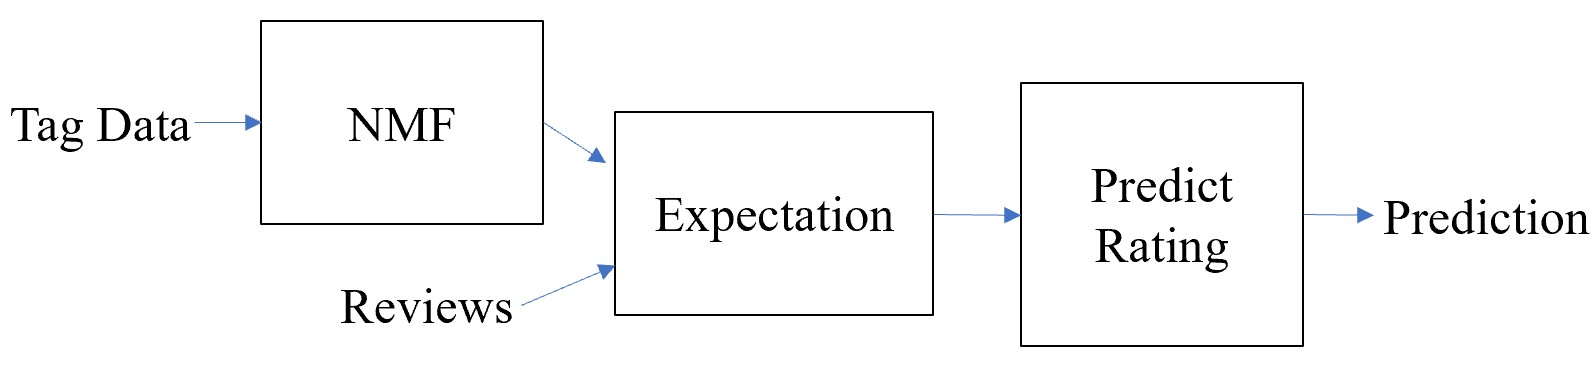
\includegraphics[scale=0.5]{./figs/blockdiagram.jpg}
   \caption{Block diagram of proposed system.}
\end{figure}

The overall architecture for our system is shown in Figure 1.

\subsection{Nonnegative Matrix Factorization}

We begin with the tag data, stored as a matrix of $t$ rows and $m$ columns. Here, $t$ is the number of tags and $m$ is the number of movies in the dataset.
We perform NMF on the tag data matrix with 50 templates, which gives us a template matrix $W$ and an activation matrix $H$.
In W, we have $t$ rows and $R$ columns, where $R$ represents the number of templates. In $H$, we have $R$ rows and $m$ columns. 

Each template is comprised of clusters of tags and represents a genre. For example, the romantic comedy genre might contain the tags "cliché," "romance," "Ryan Gosling," and "comedy." In $H$, each movie is broken down into its component genres.

It is important to mention that we use a random initialization. Ideally, we would want to discount negative tags by setting corresponding entries in the $W$ initialization to 0 (so that if someone happened to love some movies that were tagged "not funny," they would not express a preference towards other "not funny" movies). However, this task is challenging because it requires either manually reviewing each of the 1,128 tags or performing some sort of sentiment analysis. Thus we make the (perhaps dangerous) assumption that there are not too many negative tags, or that the negative tags are mainly associated with movies with low ratings.

One of the parameters we tried to vary was the number of templates used. However, performance did not improve significantly when using 50, 200, 500, or 1000 templates. By contrast, it drastically increased the runtime. We also noticed that between 10 and 50 templates, there was a small but noteworthy increase in performance and not a significant increase in runtime, so we decided to use 50 templates.

\subsection{Expectation}

Next, we assemble a new matrix of reviews. This matrix has $m$ rows and $p$ columns, where $p$ is the number of reviewers, and stores all ratings made by each user.

Then, we create another matrix $M$, which represents each reviewer's affinity to each genre. 
$M$ has $R$ rows and $p$ columns. Each entry in $M$ is an rating out of five stars indicating what a reviewer is expected to rate a typical movie from a given genre.
We get this information by taking the "expectation" of all the reviewer's ratings. In this expectation, ratings of movies more relevant to the genre of interest (as defined in $H$) are given more weight.

\subsection{Predict Rating}
Finally, we generate a predicted rating for a movie and reviewer from a query. For example, suppose we want to predict what reviewer A will rate the movie \textit{La La Land}. To do this, we will use a "genre fingerprint" for our movie.

Recall that $H$ is an $R \times m$ matrix, representing the relevance of each genre to each movie. We can $L1$ normalize the columns of $H$ to create a matrix storing the genre fingerprints of each movie.
These fingerprints indicate the breakdown of the movie into its component genres, such that each genre represents a proportion of the entire movie. See Figure 2 for examples of genre fingerprints.

For our example, let's assume that \textit{La La Land}'s fingerprint is 75\% romantic comedy and 25\% drama. Then, based on reviewer A's preferences for these genres (from matrix $M$), we can generate a preliminary prediction for their rating.

Finally, we look at the mean movie rating for \textit{La La Land}. If this mean rating is higher than our preliminary prediction, we round up to the nearest half-star. Otherwise, we round down.

\section{RESULTS}

For our experiments, we use the ratings from the first 1,024 movies from the MovieLens dataset and the relevance of those movies to each of the 1,128 tags. The 204,924 available ratings were divided into an 80\% training and 20\% testing split, and the system was applied to the training cases to make predictions for test cases \cite{lenskitmodule}. As is common in CF problems, we use the Root Mean Square Error (RMSE) as an evaluation metric \cite{lenskitmodule}. RMSE is calculated as follows: 
$$\sqrt{\frac{\sum_{i=1}^N (x_i - \hat{x}_i)^2}{N}},$$
where $N=40,984$ is the number of ratings in the testing set, $x_i$ is the actual rating, and $\hat{x}_i$ is our predicted rating.

Note that the training and test splits are randomized, but we will share results for one particular instance, and the predictions should relatively be the same throughout different instances. As a baseline, the RMSE when predicting the mean movie rating was 0.9644. Originally, before implementing the rounding mechanism, the RMSE with our algorithm was about 0.9748. We noticed that even the RMSE with the mean was better, but thought that our system was considering different factors--namely, the tags. Additionally, we suspected there could be some error if, for example, we predicted 3.6 stars as a rating but the true rating was 3.5 stars. Thus, we decided to round our prediction using the mean as an indicator. After adding the rounding, the RMSE decreased to approximately 0.9597. 

There are a few observations we can make about these results. First, we can study the genre fingerprint for the most and least accurate predictions. More specifically, the difference between our predicted rating and the true rating was 0 stars for the accurate rating, and 4 stars for the inaccurate rating. Referencing Figure 2, we notice that in the case of the accurate rating, the most prominent genre represents about 30\% of the movie, and all other genres comprise 15\% or less. On the other hand, for the inaccurate rating, the most prominent genre only represents about 14\% of the movie, and there are five other smaller peaks between 8\% and 10\% alone.

\begin{figure}[h]
   \begin{subfigure}[b]{\columnwidth}
      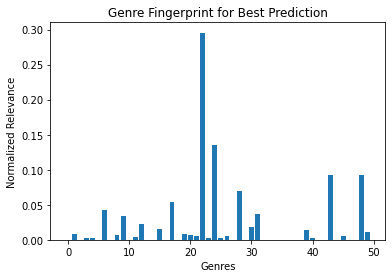
\includegraphics[width=\linewidth]{./figs/bestfingerprint.png}
      \caption{Fingerprint of movie from good prediction.}
   \end{subfigure}
   \hfill
   \begin{subfigure}[b]{\columnwidth}
      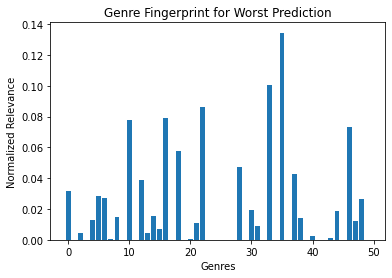
\includegraphics[width=\linewidth]{./figs/worstfingerprint.png}
      \caption{Fingerprint of movie from bad prediction.}
   \end{subfigure}
   \caption{Fingerprints of two movies. A fingerprint is the breakdown of the movie into genres. We can see that the fingerprint of the movie from the bad prediction has a wider distribution.}
\end{figure}

From Figure 2, we hypothesize that our system performs better when a movie's categorization is more straightforward, and it falls primarily into a single genre. If the movie breaks down into several genres, it is more difficult to predict a rating. What if there are two high peaks, and the reviewer loves one of the genres and hates the other one? In this case, our system would predict a medium review, but it is more likely that the reviewer would either give a high or a low rating. We attempted to address this concern by only using the most significant genre, but this approach had a very high RMSE of approximately 1.003. This failure is potentially because the true rating could just as easily reflect the secondary or tertiary genre of a movie, rather than the primary one.

Although we considered filtering the genres by a certain relevance, the variation in normalized relevance made this problematic. Instead, we tried filtering tags. If the total tag relevance across all movies was under a certain amount, we ignored that tag by setting its initialization in the $W$ matrix to 0 for NMF. Running our algorithm with this adjustment gave an RMSE of about 0.9739, which was approximately the same as running without this adjustment. One reason this filtration was not effective might be because the relevance of the tags does not matter as much as their meaning. As mentioned previously, another step could be to filter negative tags.

Besides the genre fingerprint, we can look at the distribution of ratings across all reviewers for these accurate and inaccurate predictions. Referencing Figure 3, we can see that for the "good prediction," there is a clear peak at 3 stars. As you might expect, both our predicted rating and the true ratings were 3 stars. If we look at the "bad prediction," there are peaks at 4 and 5 stars. We predict a rating of 4.5 stars, which seems to be reasonable. However, the reviewer in question gave a 0.5 star rating.

\begin{figure}[h]
   \begin{subfigure}[b]{\columnwidth}
      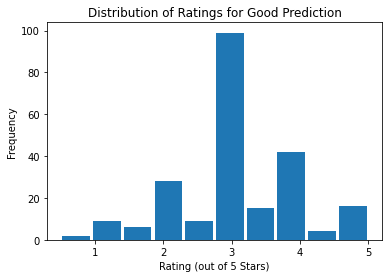
\includegraphics[width=\linewidth]{./figs/gooddist.png}
      \caption{Distribution of ratings for a well-predicted movie. The predicted and true ratings were both 3.0 stars.}
   \end{subfigure}
   \hfill
   \begin{subfigure}[b]{\columnwidth}
      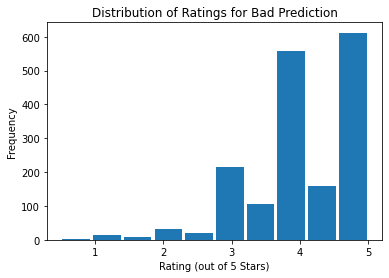
\includegraphics[width=\linewidth]{./figs/baddist.png}
      \caption{Distribution of ratings for a badly-predicted movie. The predicted and true ratings were 4.5 and 0.5 stars respectively, while the most popular ratings seem to have been 4.0 and 5.0 stars.}
   \end{subfigure}
   \caption{Rating distributions for two movies.}
\end{figure}

From Figure 3, we hypothesize that there may be anomalies or outliers in our system. Because the RMSE gives more weight to large prediction errors, we can see the results of these anomalies in our error.

Ultimately, these observations may illustrate that tag data is only one indicator of what someone might rate a movie. This dependency is a major drawback of our system, as compared to other systems that use several and hence have lower RMSEs. For example, a study looking more in-depth on temporal effects obtained an RMSE of 0.8784 \cite{netflix}. We do know, however, that an RMSE of between 0.85 and 1.3 or more is to be expected when predicting ratings \cite{netflix}.


\section{CONCLUSION}
Hybrid approach

\bibliographystyle{IEEEtran}
\bibliography{paperbib}




\end{document}
